%!TEX root = ../Main.tex

\begin{figure}

\begin{center}
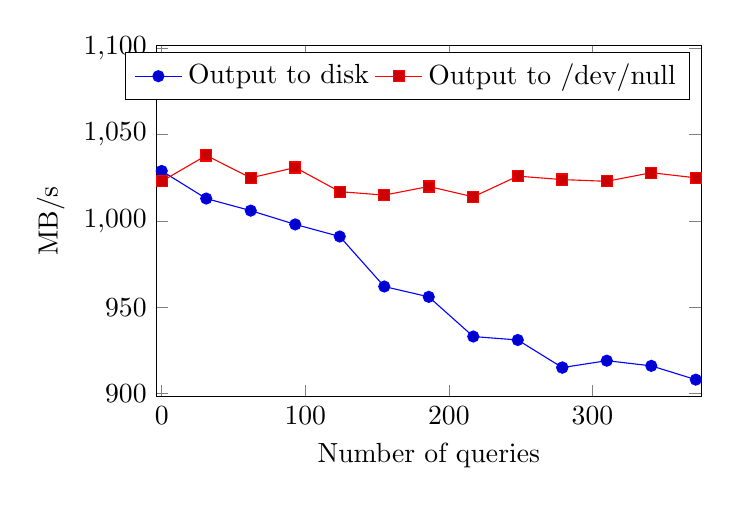
\begin{tikzpicture}
\begin{axis}[
	x tick label style={/pgf/number format/1000 sep=},
	ylabel=MB/s,
  ymin=900, ymax=1100,
%  xmax=372,
  xlabel=Number of queries,
	enlargelimits=0.01,
	legend style={legend columns=-1},
  width=8.5cm, height=6.05cm,
%	legend style={at={(0.5,-0.1)},anchor=north,legend columns=-1},
%	ybar interval=0.7,
]

% bench/raw.txt
% Running with fewer queries
% \addplot coordinates {(0,1025.5) (1,1029.6) (48,978) (96,941) (144,943) (192,936) (240,904) (276,895.5) (324,881) (372,846.2) };

% bench/raw.txt
% Running with fewer queries, better distribution
% \addplot coordinates { (0,1029) (31,1013) (62,1006) (93,998) (124,991) (155,941) (186,956) (217,933) (248,931) (279,915) (279,915) (310,919) (341,916) (372,908) };

%% APPLY LOPASS
\addplot coordinates { (0,1029) (31,1013) (62,1006) (93,998) (124,991) (155,962) (186,956) (217,933) (248,931) (279,915) (279,915) (310,919) (341,916) (372,908) };


% Fusion, no output
% \addplot coordinates { (0,1001) (31,1038) (62,1025) (93,1031) (124,1006) (155,1015) (186,1020) (217,997) (248,1026) (279,1024) (310,1009) (341,1038) (372,1025) };

%% APPLY LOPASS
\addplot coordinates { (0,1023) (31,1038) (62,1025) (93,1031) (124,1017) (155,1015) (186,1020) (217,1014) (248,1026) (279,1024) (310,1023) (341,1028) (372,1025) };

% No fusion, no output
% \addplot coordinates { (0,987) (31,1037) (62,1024) (93,1002) (124,1037) (155,1024) (186,1004) (217,1040) (248,1023) (279,998) (310,1018) (341,1013) (372,1003) };

\legend{Output to disk, Output to /dev/null};

\end{axis}
\end{tikzpicture}
\end{center}


\caption{Decrease in read throughput as queries are added, comparing writing the output to disk and writing to /dev/null.}
\label{icicle:fig:bench:queries}
\end{figure}


% \begin{figure}
% \begin{tikzpicture}
% \begin{axis}[
% 	x tick label style={/pgf/number format/1000 sep=},
% 	ylabel=MB/s,
%   ymin=0, ymax=1200,
%   xlabel=Number of threads,
% 	enlargelimits=0.01,
% 	legend style={legend columns=-1},
% ]
% \addplot coordinates { (1,163) (2,335) (3,442) (4,532) (5,578) (6,615) (7,633) (8,628) (9,631) (10,626) (11,637) (12,643) (13,658) (14,795) (15,781) (16,798) (17,840) (18,864) (19,862) (20,867) (21,847) (22,877) (23,876) (24,884) (25,862) };
% \end{axis}
% \end{tikzpicture}
% \caption{Scaling as threads are added}
% \label{icicle:fig:bench:scaling}
% \end{figure}


